\documentclass[../main.tex]{subfiles}
\begin{document}

\section{Categorical Variables Conditioned on Categorical Distributions}

Categorical data can be likened to set measurement, where each category is a set
and researchers often want to know how many members each set has and what
intersections are common between sets \cite{agresti_categorical_2011,schneider_set-theoretic_2012}
  It is the latter that is analogous to a
conditional probability, the question of the likelihood of membership in one
set given membership in another. And sometimes there is also a quantitative
component involved too. The most common approach is usually to create a list of frequencies, sometimes of sets of one category or a cross-table\cite{goodman_measures_1991} which is an aggregate function applied to the product of two or more sets.

 While a table is encouraged for a small number of variables
 \cite{munzner_what:_2014}), bar graphs and histograms are typically used to display differences between subsets \cite{ioannidis_history_2003-1, friendly_brief_2006}. Variations on histograms
 include the hanging rootgram, ord plot, and other distribution oriented
 plots \cite{tukey_exploratory_1977, friendly_visualizing_2000}. While conditional  distributions can somewhat be visualized using Fourfold displays, Mosaic displays, and using logit regression models, these plots have somewhat limited dimensionality and are somewhat limited to 3 sets of categories
 \cite{friendly_visualizing_2000}. 
   
 
\begin{figure}
  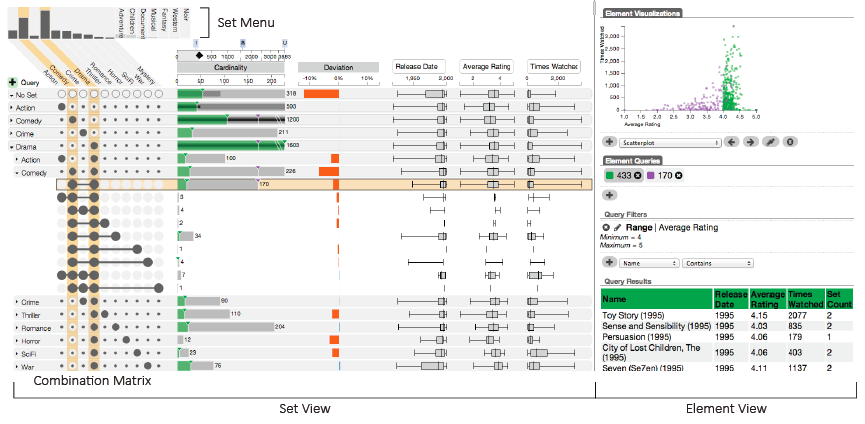
\includegraphics[width=\textwidth]{upsetfig1}
   \caption{UpSet dashboard displaying the relationships amongst movie genres. On the left is the set visualization; the columns are the sets and
   the rows are the exclusive intersections or aggregates. On the right is the element view, and the scatter plot is a comparison of two sets with each dot equaling one element in the set.}
   \label{fig:upsetfig}
\end{figure}

The UpSet tool is designed to display a much larger number of set intersections and the aggregate information of quantitative attributes and set membership. \cite{lex_upset:_2014} As shown in figure~\ref{fig:upsetfig}, the Upset tool provides linked set and element views. The set view provides the intersections and their
aggregates, the frequencies of each set and intersection, and the aggregate
statistics of the associated quantitative variables, while the element view shows
selected elements and information about their set membership. The set view yields the distributions of each of the attributes. Far example the selected row (in the gray box) are the distributions of each quantative variable in the comedy set. Every row underneath is the distribution of that quantative variable restricted to movies in the intersection of the selected sets. For example, the distribution of ratings of movies that are both comedies and dramas. The Upset tool
also facilitates comparison of filtered sets via scatterplot, which acts as a
visualization of the attributes of the data conditioned on membership in the
filtered set.  

\end{document}
